\documentclass[11pt]{article}

% This template is intentionally simple so it compiles cleanly on Overleaf and
% can be adapted to the journal submission system without a custom class file.
\usepackage[a4paper,margin=1in]{geometry}
\usepackage[T1]{fontenc}
\usepackage[utf8]{inputenc}
\usepackage{lmodern}
\usepackage{microtype}
\usepackage{graphicx}
\usepackage{caption}
\usepackage{booktabs}
\usepackage{array}
\usepackage{amsmath,amssymb}
\usepackage{caption}
\usepackage{enumitem}
\usepackage{xcolor}
\usepackage{multirow}
\usepackage[colorlinks=true,linkcolor=black,citecolor=black,urlcolor=black]{hyperref}
\usepackage[nameinlink,noabbrev]{cleveref}

\graphicspath{{figures/}}
\setlength{\parindent}{0pt}
\setlength{\parskip}{0.7em}

\DeclareCaptionLabelSeparator{naturebar}{\space|\space}
\captionsetup{
  font=small,
  labelfont=bf,
  labelsep=naturebar,
  singlelinecheck=false
}
\captionsetup[figure]{name={Supplementary Fig.}}
\captionsetup[table]{name={Supplementary Table}}

\renewcommand{\thefigure}{\arabic{figure}}
\renewcommand{\thetable}{\arabic{table}}
\renewcommand{\theequation}{S\arabic{equation}}

% Make cross-references match Nature-style supplementary labels.
\crefname{figure}{Supplementary Fig.}{Supplementary Figs.}
\Crefname{figure}{Supplementary Fig.}{Supplementary Figs.}
\crefname{table}{Supplementary Table}{Supplementary Tables}
\Crefname{table}{Supplementary Table}{Supplementary Tables}
\crefname{equation}{Supplementary Eq.}{Supplementary Eqs.}
\Crefname{equation}{Supplementary Eq.}{Supplementary Eqs.}

% Safe placeholder for showing includegraphics commands inside framed boxes.
\newcommand{\placeholdergraphics}[1]{%
  {\ttfamily\small \textbackslash includegraphics[width=\textbackslash linewidth]\{\detokenize{#1}\}}%
}

\newcommand{\manuscripttitle}{[Full manuscript title]}
\newcommand{\correspondingauthor}{[Corresponding author name and email]}
\newcommand{\suppdoi}{[Optional manuscript DOI or tracking number]}

% Make unnumbered sections appear in the table of contents.
\newcommand{\suppsection}[1]{%
  \phantomsection
  \section*{#1}
  \addcontentsline{toc}{section}{#1}
}

\newcommand{\suppsubsection}[1]{%
  \phantomsection
  \subsection*{#1}
  \addcontentsline{toc}{subsection}{#1}
}

\renewcommand{\contentsname}{Contents}

\title{\vspace{-2em}Supplementary Information\\[0.5em]
\large \manuscripttitle}
\author{[Author One] \and [Author Two] \and [Author Three]}
\date{}

\begin{document}
\maketitle

\begin{center}
\textbf{Correspondence:} \correspondingauthor\\
\textbf{Manuscript identifier:} \suppdoi
\end{center}

\vspace{1.5em}

\tableofcontents

\clearpage

\suppsection{Additional TFI observable estimation}

In the main text, longitudinal spin correlations are used as representative observables to demonstrate same-size generation, cross-scale generation and thermodynamic-limit inference in the transverse-field Ising model. Here we provide additional estimated observable results for the 10-qubit transverse-field Ising model to assess whether Diffushadow-generated classical shadows preserve information beyond the observables emphasized in the main figures. We consider local spin correlations, non-local \(X\)-string observables and the ground-state energy, thereby providing a broader validation of the generated measurement data.



\begin{figure}[htbp]
  \centering
  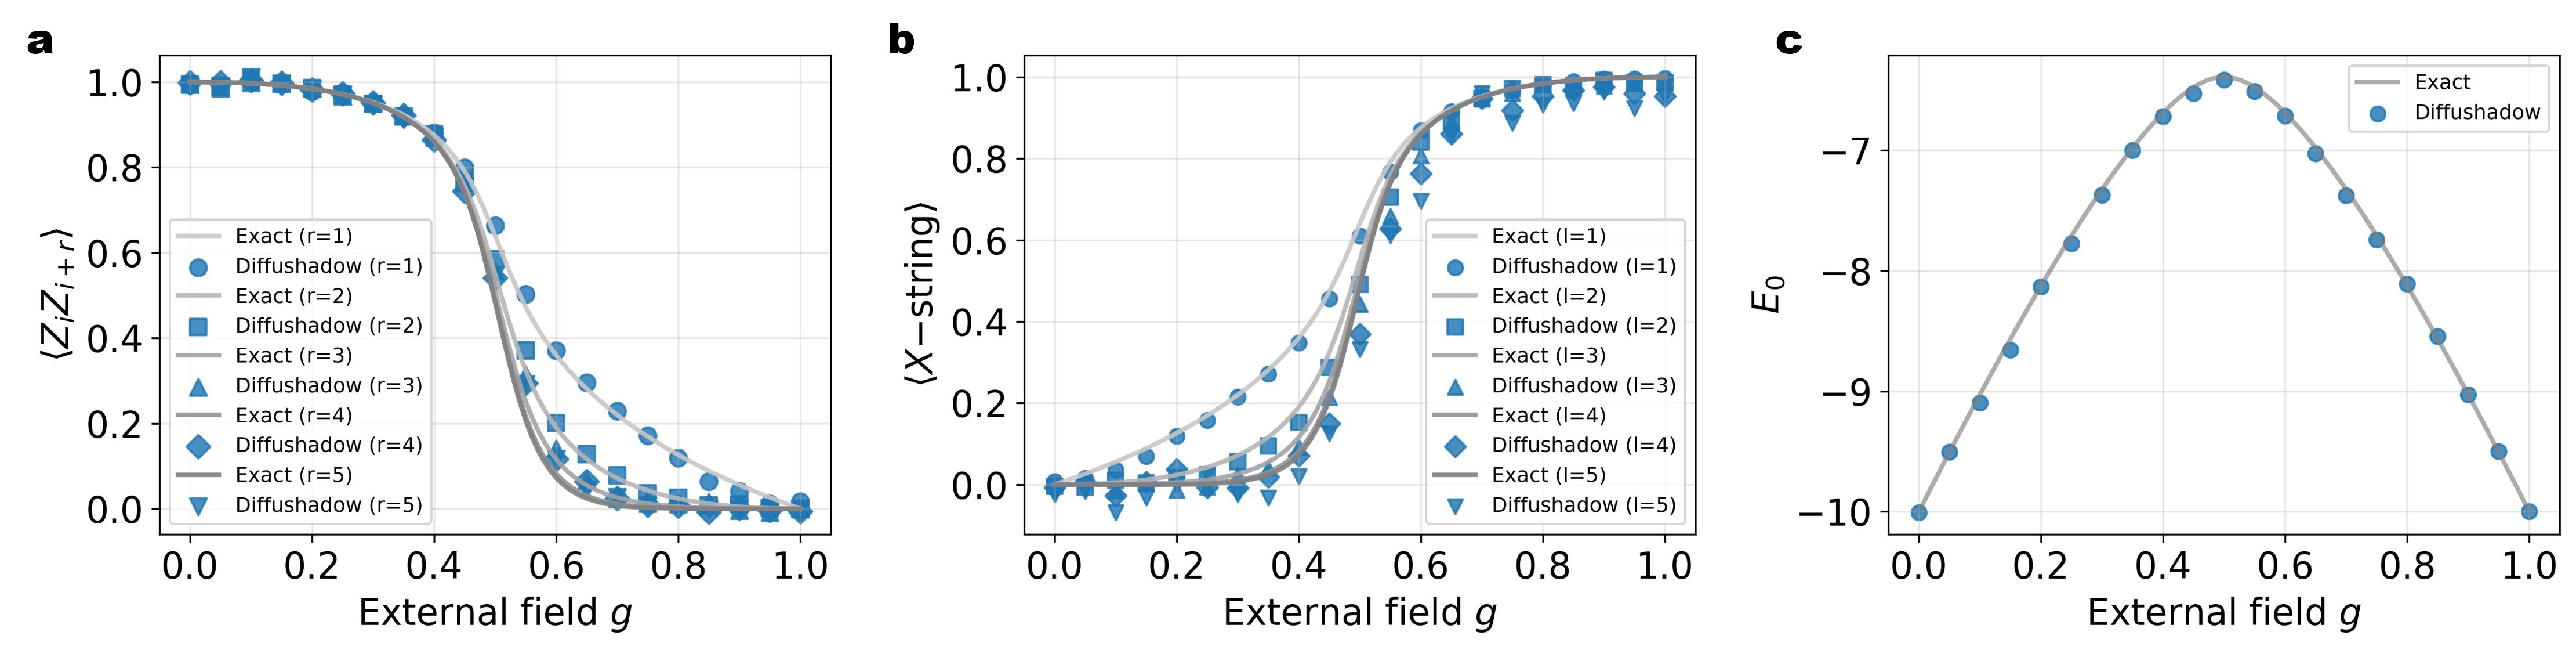
\includegraphics[width=\textwidth]{figures/Figure_10q_all.png}
  \caption{Additional observable estimation in the transverse-field Ising model. 
Ground-state observables of the 10-qubit transverse-field Ising model estimated from Diffushadow-generated classical-shadow measurements. 
(a) Two-point spin correlations \(\langle Z_i Z_{i+r}\rangle\) for different correlation distances \(r\). 
(b) \(X\)-string order parameters with different string lengths \(\ell\). 
(c) Ground-state energy \(E_0\). 
Grey solid curves denote exact diagonalization results, and blue markers denote estimates obtained from Diffushadow-generated classical-shadow measurements. 
In panels a and b, marker shapes distinguish the correlation distance \(r\) and the string length \(\ell\), respectively. 
These additional observables complement the longitudinal spin-correlation results emphasized in the main text and show that Diffushadow-generated shadows support estimation of both local correlations, extended string observables and the ground-state energy.}
  \label{fig:TFI_10q_all}    
\end{figure}



Supplementary Fig.~\ref{fig:TFI_10q_all} compares observable estimates obtained from Diffushadow-generated classical-shadow measurements with exact diagonalization results. We consider three representative ground-state observables of the 10-qubit transverse-field Ising model, including the two-point spin correlations \(\langle Z_i Z_{i+r}\rangle\), the \(X\)-string order parameters with different string lengths \(\ell\), and the ground-state energy \(E_0\). The two-point correlations probe the longitudinal spin-order structure, the \(X\)-string observables test whether the generated shadows preserve information about more extended non-local operators, and the ground-state energy provides an aggregate Hamiltonian-level quantity estimated from the generated measurement data. 
Diffushadow estimates closely follow the exact curves across the transverse-field parameter \(g\). For the two-point correlations, the generated-measurement estimates reproduce the decay of longitudinal spin correlations as the system moves from the ferromagnetic regime to the paramagnetic regime. For the \(X\)-string observables, Diffushadow captures the complementary increase of string-order signals with increasing transverse field. The ground-state energy is also accurately recovered from the generated shadows, showing that the generated measurement samples preserve information not only about individual correlation functions but also about an aggregate Hamiltonian-level observable.




\begin{table}[htbp]
\centering
\small
\caption{MSE of selected observable estimates for the 10-qubit transverse-field Ising model. The table reports the ground-state energy \(E_0\) and representative \(X\)-string observables; \(ZZ\) correlations are omitted to avoid redundancy with the main text. ShGPT denotes ShadowGPT, Diffu-rdm denotes Diffushadow with randomly selected decoding positions, Diffu-s1 denotes one-step Diffushadow decoding, and Diffu denotes the full Diffushadow with entropy-based iterative decoding.}
\label{tab:mse_table}
\begin{tabular}{llcccc}
\hline
 &Model & $E_0$ & $\left(\prod_{i=1}^1 X_i\right)$ & $\left(\prod_{i=1}^3 X_i\right)$ & $\left(\prod_{i=1}^5 X_i\right)$\\
\hline
\multirow{4}{*}{$g=0.1$} 
& ShGPT      & $3.63{\times}10^{-4}$ & $7.56{\times}10^{-4}$ & $6.80{\times}10^{-4}$ & $2.77{\times}10^{-3}$\\
& Diffu-rdm & $2.34{\times}10^{-3}$ & $2.90{\times}10^{-4}$ & $1.88{\times}10^{-6}$ & $3.69{\times}10^{-3}$\\
& Diffu-s1  & $7.99{\times}10^{1}$ & $1.92{\times}10^{-4}$ & $1.16{\times}10^{-4}$ & $\underline{\mathbf{4.10{\times}10^{-4}}}$\\
& \textbf{Diffu}    & $\underline{\mathbf{2.77{\times}10^{-4}}}$ & $\underline{\mathbf{2.20{\times}10^{-4}}}$ & $\underline{\mathbf{1.85{\times}10^{-7}}}$ & $1.33{\times}10^{-3}$\\
\hline
\multirow{4}{*}{$g=0.5$} 
& ShGPT      & $1.35{\times}10^{-2}$ & $6.31{\times}10^{-5}$ & $2.15{\times}10^{-4}$ & $2.77{\times}10^{-4}$\\
& Diffu-rdm & $7.59{\times}10^{-3}$ & $2.17{\times}10^{-4}$ & $6.00{\times}10^{-4}$ & $1.12{\times}10^{-2}$\\
& Diffu-s1  & $1.00{\times}10^{1}$ & $1.05{\times}10^{-4}$ & $5.82{\times}10^{-2}$ & $1.71{\times}10^{-1}$\\
& \textbf{Diffu}    & $\underline{\mathbf{7.13{\times}10^{-3}}}$ & $\underline{\mathbf{4.01{\times}10^{-5}}}$ & $\underline{\mathbf{4.90{\times}10^{-5}}}$ & $\underline{\mathbf{2.29{\times}10^{-4}}}$\\
\hline
\multirow{4}{*}{$g=0.9$} 
& ShGPT      & $6.79{\times}10^{-4}$ & $9.88{\times}10^{-6}$ & $4.76{\times}10^{-5}$ & $\underline{\mathbf{7.57{\times}10^{-5}}}$\\
& Diffu-rdm & $5.05{\times}10^{-4}$ & $6.57{\times}10^{-8}$ & $6.20{\times}10^{-4}$ & $4.28{\times}10^{-3}$\\
& Diffu-s1  & $1.47{\times}10^{-3}$ & $4.44{\times}10^{-6}$ & $4.33{\times}10^{-4}$ & $1.21{\times}10^{-3}$\\
& \textbf{Diffu}    & $\underline{\mathbf{4.98{\times}10^{-4}}}$ & $\underline{\mathbf{3.32{\times}10^{-6}}}$ & $\underline{\mathbf{2.22{\times}10^{-8}}}$ & $3.88{\times}10^{-4}$\\
\hline
\end{tabular}
\end{table}

We further provide quantitative comparisons in Supplementary Table~\ref{tab:mse_table}. Because \(ZZ\) correlations are already used as the main observables in the main text, the quantitative table here focuses on the ground-state energy and representative \(X\)-string observables to avoid redundancy. The table reports mean squared errors at \(g=0.1\), \(g=0.5\) and \(g=0.9\), comparing the autoregressive ShadowGPT baseline with several Diffushadow decoding variants. Diffu-rdm denotes iterative decoding with randomly selected positions, Diffu-s1 denotes one-step decoding, and Diffu denotes the full entropy-based iterative decoding strategy. The one-step variant shows substantially larger errors, especially for the ground-state energy, confirming the importance of iterative denoising. Random position selection can perform competitively for some individual observables, but is less consistent than the full entropy-based strategy. Overall, full Diffushadow achieves low errors across representative observables and provides a stable alternative to sequential autoregressive generation.






\suppsection{Effect of the number of denoising steps}


\begin{figure}[htbp]
  \centering
  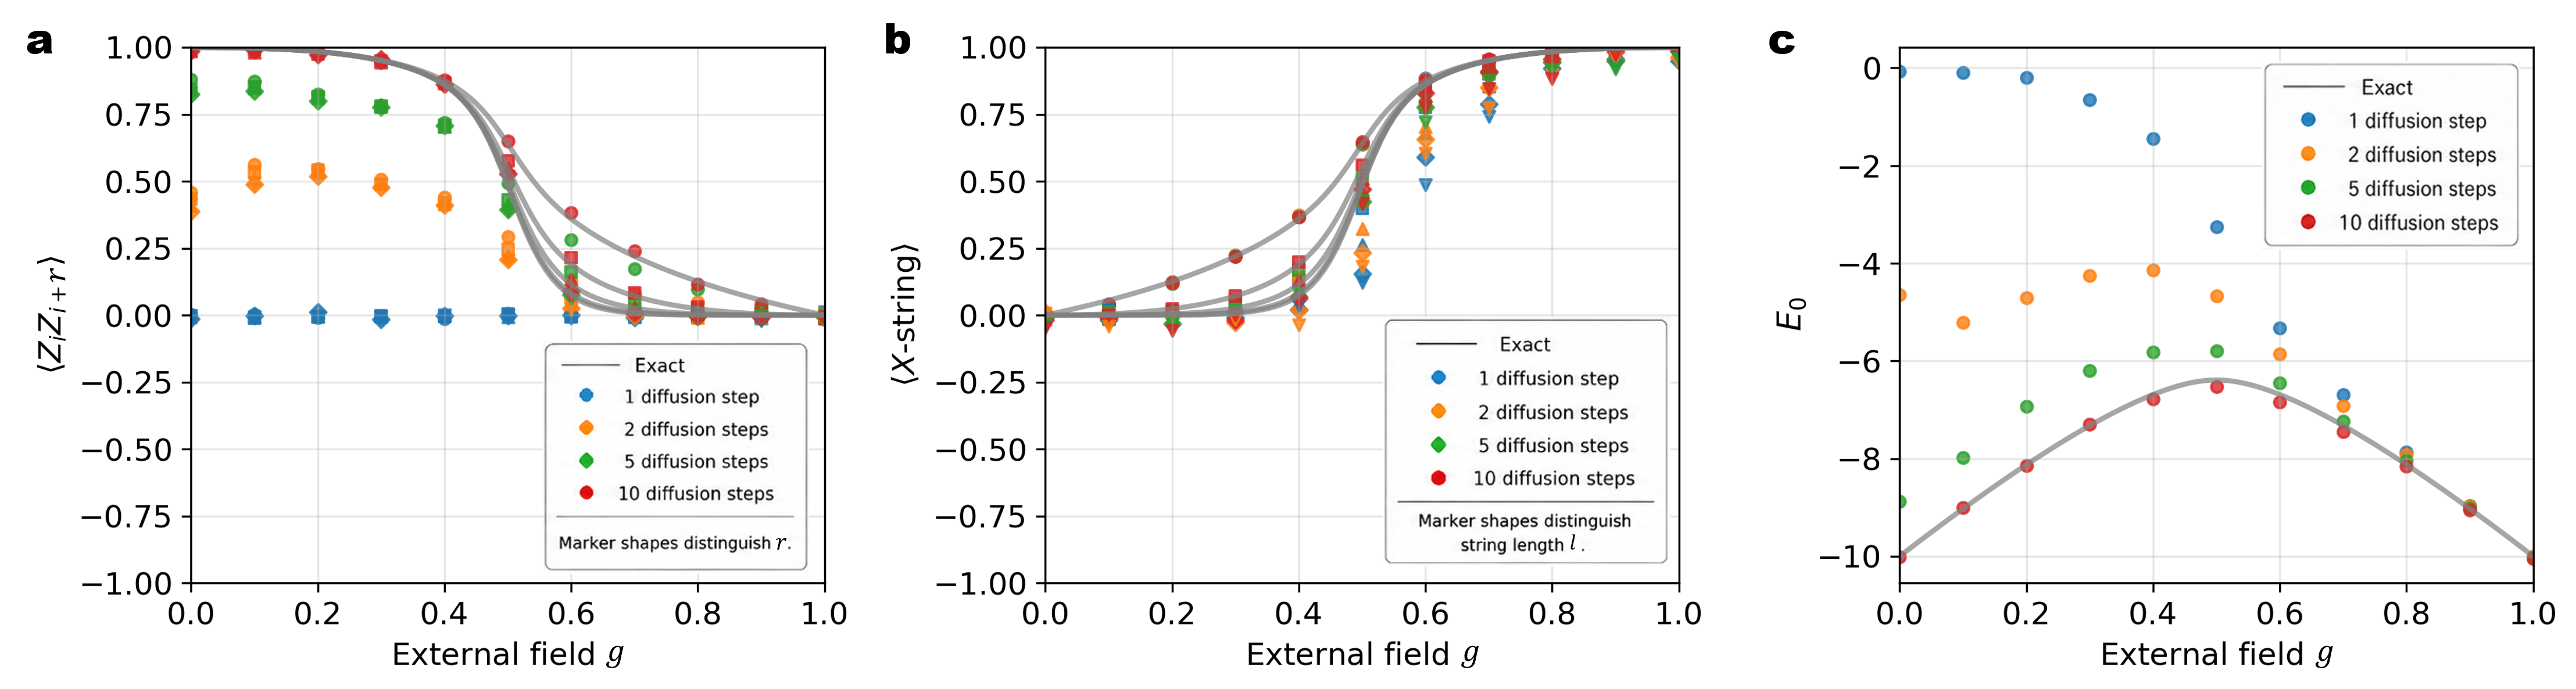
\includegraphics[width=\textwidth]{figures/Figure_diffusion_steps1.2.png}
  \caption{Effect of denoising steps on observable estimation in the transverse-field Ising model. 
Physical observables of the 10-qubit transverse-field Ising model estimated from Diffushadow-generated classical-shadow measurements using different numbers of denoising steps. 
(a) Two-point spin correlations \(\langle Z_i Z_{i+r}\rangle\). 
(b) \(X\)-string order parameters with different string lengths \(\ell\). 
(c) Ground-state energy per site \(E_0/N\). 
Grey solid curves denote exact diagonalization results, and colored markers denote Diffushadow estimates generated with 1, 2, 5 and 10 denoising steps. 
In panel a, marker shapes distinguish the correlation distance \(r\); in panel b, marker shapes distinguish the string length \(\ell\). 
Increasing the number of denoising steps improves the agreement between generated-measurement estimates and exact results, with one-step decoding showing the largest deviation and 10-step denoising giving the most accurate estimates.}
  \label{fig:diffusion_steps}    
\end{figure}


We further examine how the number of denoising steps affects observable estimation from Diffushadow-generated classical shadows. In the generation process, Diffushadow starts from a fully masked measurement-outcome sequence and progressively unmasks predicted outcomes. The number of denoising steps controls the trade-off between generation efficiency and iterative refinement. Fewer steps unmask more positions at each iteration and therefore reduce generation time, whereas more steps allow the model to reveal high-confidence positions more gradually and condition later predictions on previously generated outcomes. We evaluate this effect using the 10-qubit transverse-field Ising model.

Supplementary Fig.~\ref{fig:diffusion_steps} shows observable estimates obtained with different numbers of denoising steps. One-step decoding leads to the largest deviations from the exact results, whereas increasing the number of denoising steps systematically improves the agreement with exact diagonalization. The best results are obtained with 10 denoising steps among the tested settings. This trend supports the importance of iterative refinement in Diffushadow generation. Once high-confidence measurement outcomes are unmasked, they provide additional context for predicting the remaining, more uncertain positions, leading to more accurate and physically consistent generated measurement snapshots.

The improvement from additional denoising steps is especially visible in the low-field regime \(g < 0.5\), where the transverse-field Ising ground state exhibits stronger longitudinal order and longer-range spin correlations. In this regime, accurately generating globally consistent measurement outcomes requires the model to capture correlations across multiple sites, and gradual denoising provides a useful mechanism for progressively establishing these correlations. By contrast, in the high-field paramagnetic regime \(g > 0.5\), longitudinal correlations become weaker and more short-ranged, making the generated observables less sensitive to the number of refinement steps. These results indicate that multi-step denoising is particularly important for modeling ordered regimes with stronger correlation structure, while fewer steps may already be sufficient in simpler short-range-correlated regimes.





\suppsection{Effect of the number of generated classical-shadow snapshots}



We also examine how the number of generated classical-shadow snapshots affects observable estimation. In classical-shadow tomography, physical observables are estimated from a finite set of randomized measurement snapshots, and the number of snapshots \(M\) controls the sampling budget of the estimator. A larger \(M\) generally reduces sampling fluctuations, but also increases the computational cost of generation and downstream observable estimation. We therefore evaluate whether Diffushadow-generated measurements provide stable observable estimates under different sampling budgets.

Supplementary Fig.~\ref{fig:sample_size} shows results for the 10-qubit transverse-field Ising model with \(M=8{,}000\), \(10{,}000\), \(100{,}000\) and \(300{,}000\) generated snapshots, while keeping all other settings fixed. For each value of \(M\), we estimate the two-point correlations \(\langle Z_iZ_{i+r}\rangle\), \(X\)-string order parameters and the ground-state energy. Across the four sampling budgets, the estimates remain close to the exact diagonalization results, indicating that Diffushadow-generated snapshots support stable physical-property estimation over a broad range of \(M\).

Increasing \(M\) makes the estimated curves slightly smoother and reduces finite-sample fluctuations, as expected from classical-shadow estimation. However, even the smaller sampling budgets already recover the main observable trends, including the decay of longitudinal spin correlations, the growth of \(X\)-string observables and the ground-state energy curve. These results suggest that the agreement with exact results is not solely a consequence of using an extremely large number of generated samples, but also reflects the quality of the measurement distribution learned by Diffushadow.






\begin{figure}[htbp]
  \centering
  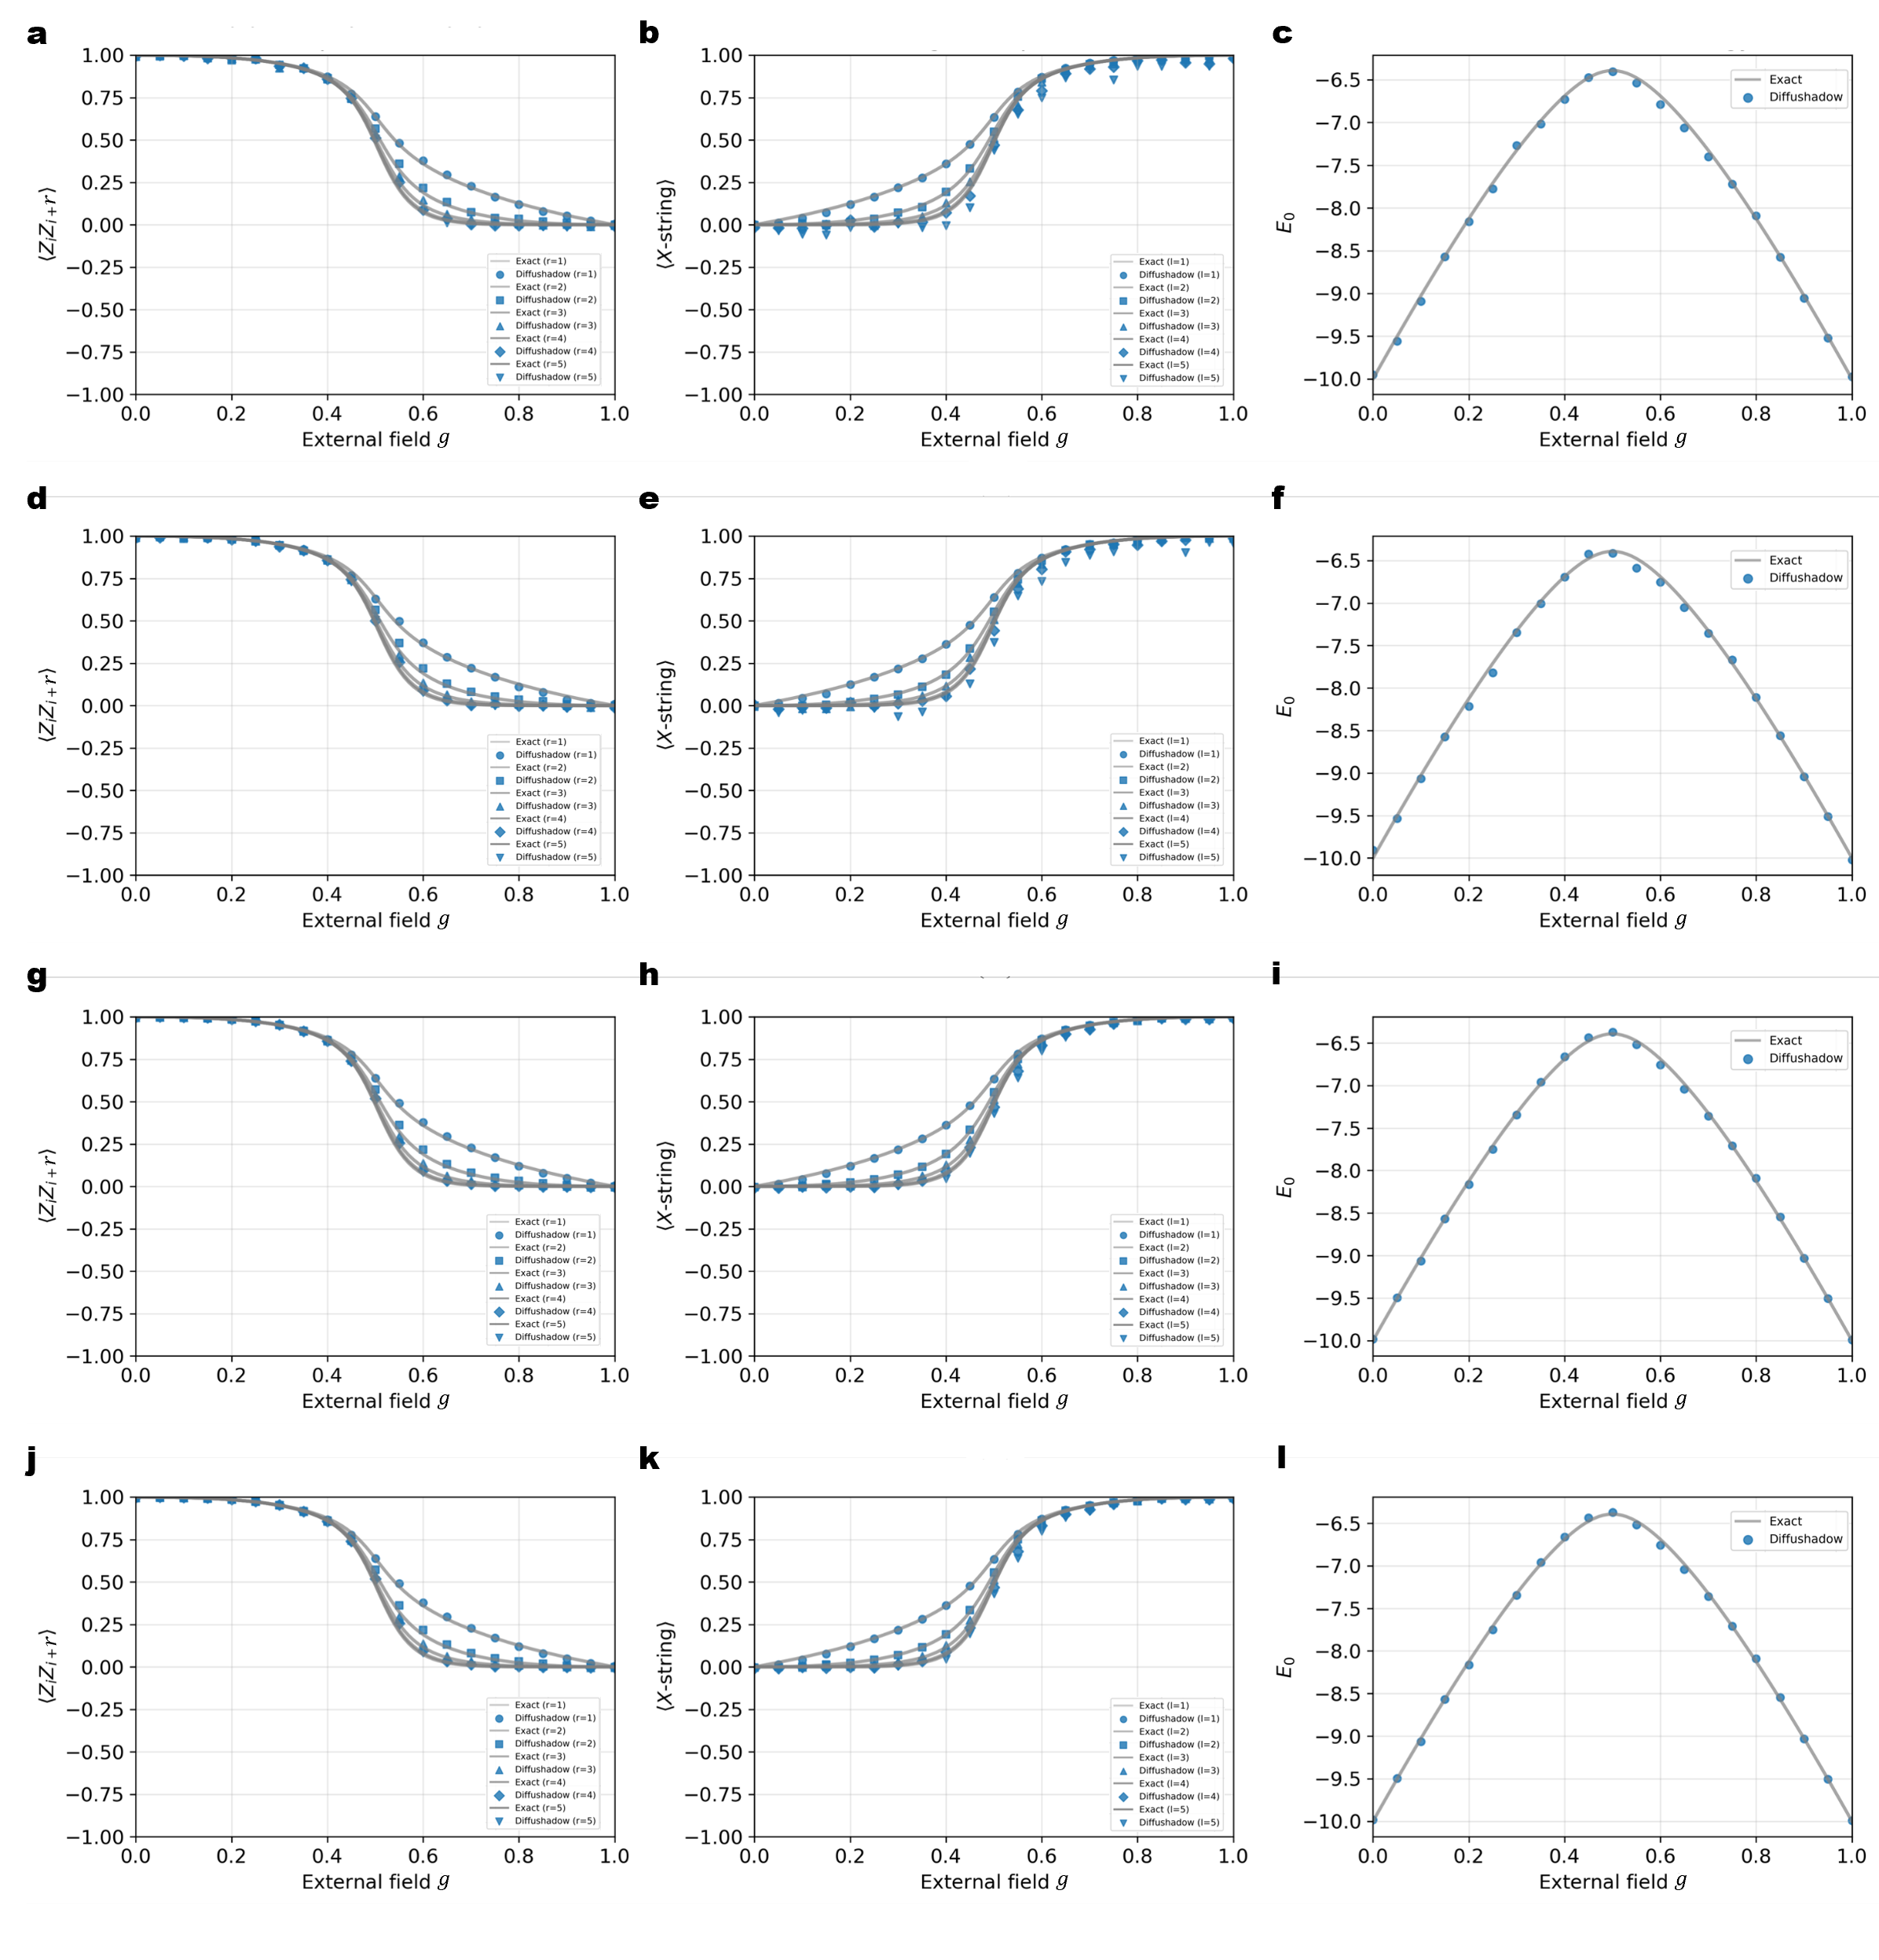
\includegraphics[width=\textwidth]{figures/Figure_sample_size1.4.png}
  \caption{Dependence of observable estimation on the number of generated classical-shadow snapshots in the transverse-field Ising model. 
Ground-state properties of the 10-qubit transverse-field Ising model estimated from Diffushadow-generated classical-shadow measurements using different numbers of generated snapshots \(M\). 
Panels a--c, d--f, g--i and j--l correspond to \(M=8\mathrm{k}\), \(10\mathrm{k}\), \(100\mathrm{k}\) and \(300\mathrm{k}\), respectively. 
In each row, the left panel shows the two-point spin correlations \(\langle Z_i Z_{i+r}\rangle\), the middle panel shows the \(X\)-string order parameters \(\langle X\text{-string}\rangle\) with different string lengths, and the right panel shows the ground-state energy per site \(E_0/N\). 
Grey solid curves denote exact diagonalization results, and blue markers denote estimates obtained from Diffushadow-generated measurements. 
In the correlation and string-order panels, different marker shapes distinguish different correlation distances \(r\) and string lengths \(l\), respectively. 
As the number of generated snapshots increases, the estimated observables remain consistently close to the exact results, indicating that Diffushadow provides stable physical-property estimation across different sampling budgets.}
  \label{fig:sample_size}    
\end{figure}



\suppsection{Stability of recursive scale extrapolation}




\begin{figure}[htbp]
  \centering
  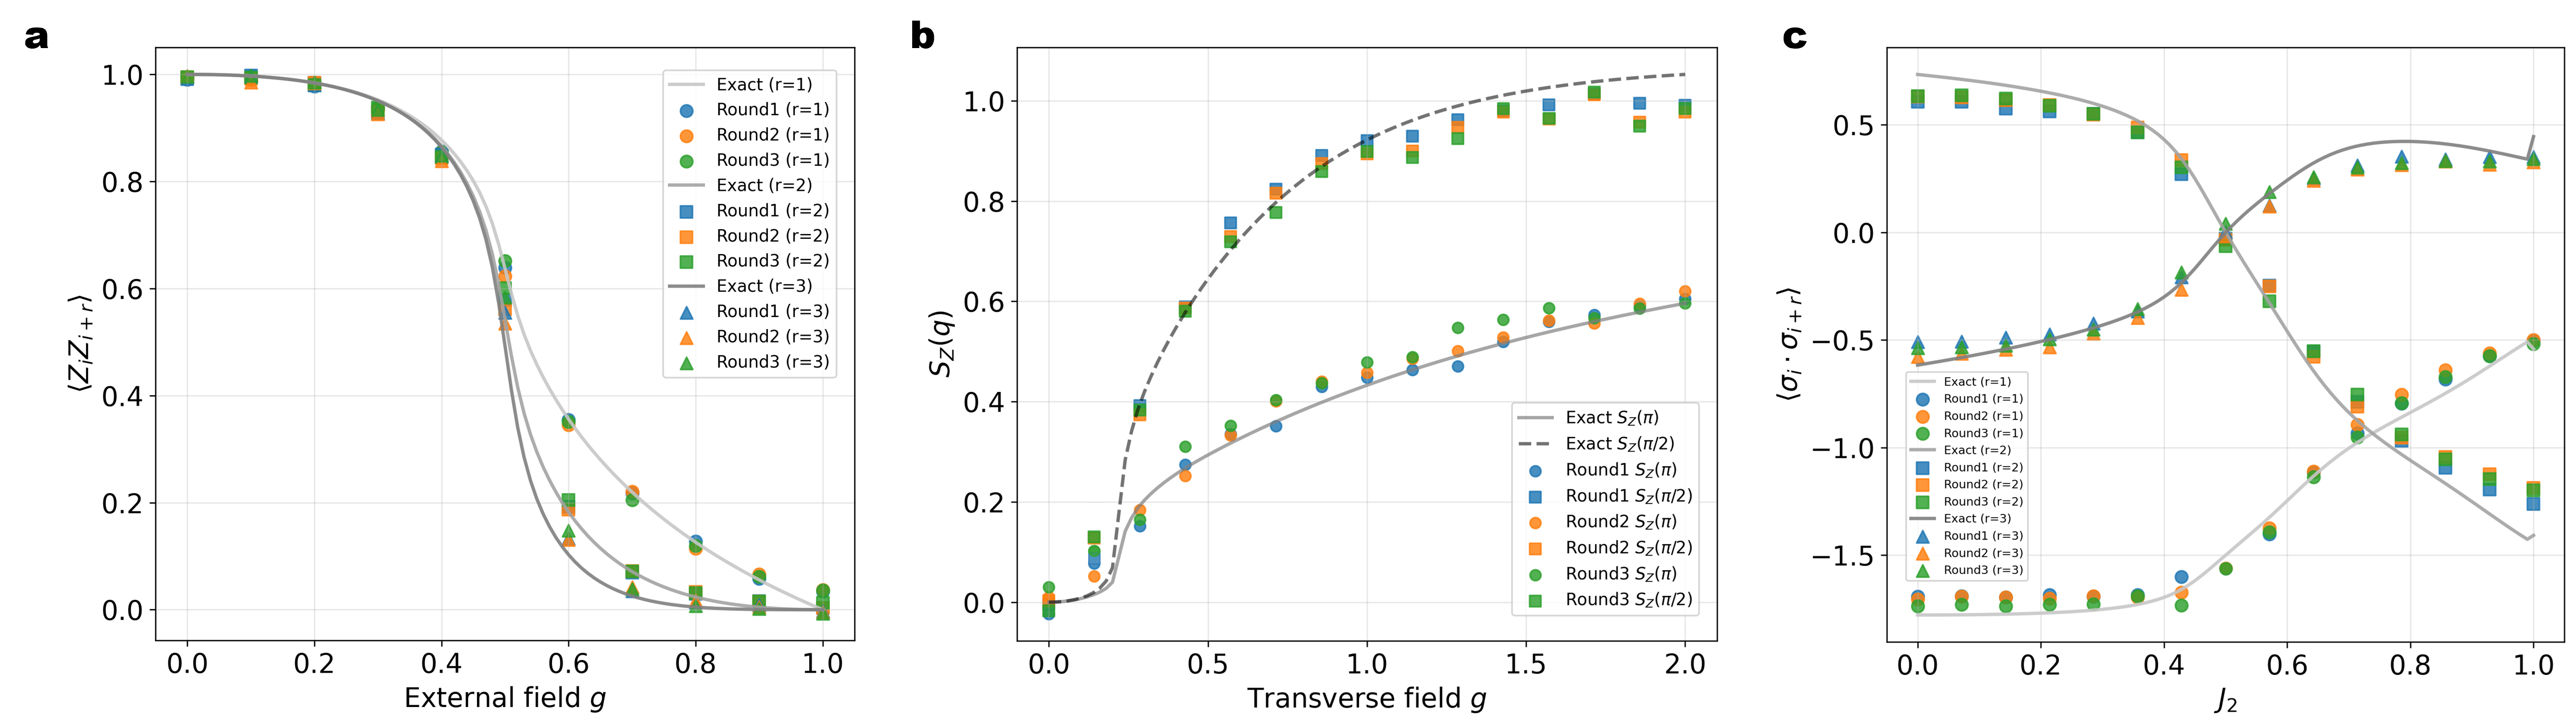
\includegraphics[width=\textwidth]{figures/Figure_stability_all2.0.png}
  \caption{Stability of recursive scale extrapolation across training rounds.
Comparison of observable estimates generated by Diffushadow models obtained from different recursive training rounds, evaluated at the same 24-qubit target system size.
(a) Transverse-field Ising spin-spin correlations \(\langle Z_i Z_{i+r}\rangle\) for \(r=1,2,3\).
(b) ANNNI structure factors \(S_Z(\pi)\) and \(S_Z(\pi/2)\).
(c) \(J_1\)-\(J_2\) spin-dot correlations \(\langle \boldsymbol{\sigma}_i\cdot\boldsymbol{\sigma}_{i+r}\rangle\) for \(r=1,2,3\).
Solid or dashed curves denote exact diagonalization results, while markers denote observables estimated from Diffushadow-generated classical-shadow measurements.
The close agreement among the three recursive rounds indicates that recursive scale extrapolation does not introduce substantial drift in the generated measurement distributions at the tested system size.}
  \label{fig:stability_analysis}    
\end{figure}

Recursive scale extrapolation progressively expands the accessible system size by incorporating generated measurements from previous rounds into subsequent training. A potential concern is that such a procedure may accumulate errors or introduce distributional drift across training rounds. To examine this issue, we compare Diffushadow models obtained from different recursive training rounds by evaluating them at the same target system size.

Supplementary Fig.~\ref{fig:stability_analysis} shows the results for 24-qubit systems generated by models from three recursive training rounds. We evaluate representative observables in the transverse-field Ising, ANNNI and \(J_1\)-\(J_2\) models. Across the three Hamiltonians, the observable estimates from different rounds remain close to one another and follow the corresponding exact results. Small deviations are observed in some parameter regions, particularly where the finite-size observables vary rapidly, but no systematic drift is observed across recursive rounds.

These results suggest that the recursive scale-extrapolation procedure is stable at the tested target size. In particular, adding generated measurements in later rounds does not substantially degrade the physical observables estimated from newly generated classical-shadow data. This supports the use of recursive training as a practical strategy for progressively extending Diffushadow to larger quantum many-body systems.


\suppsection{Classical-shadow observable estimation}


For each Hamiltonian parameter, Diffushadow generates
\(M=10{,}000\) classical-shadow measurement snapshots,
\(\mathcal{D}=\{(\mathbf{P}_t,\mathbf{b}_t)\}_{t=1}^{M}\),
where \(\mathbf{P}_t\) denotes the sequence of single-qubit Pauli
measurement bases and \(\mathbf{b}_t\) denotes the corresponding binary
measurement outcomes. The Hamiltonian parameter \(\lambda\) is evaluated
at 15 uniformly spaced values over \([0,1]\) for the TFI model,
\([0,1]\) for the \(J_1\)--\(J_2\) model, and \([0,2]\) for the ANNNI
model. Here, \(\lambda\) corresponds to \(g\), \(J_2/J_1\), and \(g\),
respectively.

The binary outcomes are mapped to Pauli eigenvalues according to
\(s_{t,i}=2b_{t,i}-1\). For uniformly sampled single-qubit Pauli
measurements, the inverse measurement channel gives the local estimator
\begin{equation}
\widehat{\sigma}^{\alpha}_{t,i}
=
3s_{t,i}\mathbf{1}[P_{t,i}=\alpha],
\qquad
\alpha\in\{x,y,z\}.
\end{equation}

For the TFI model, the translationally averaged longitudinal correlation
at distance \(r\) is estimated as
\begin{equation}
\widehat{C}_{ZZ}(r)
=
\frac{1}{MN}
\sum_{t=1}^{M}
\sum_{i=1}^{N}
\widehat{\sigma}^{z}_{t,i}
\widehat{\sigma}^{z}_{t,i+r},
\end{equation}
where all site indices are understood modulo \(N\).

For the \(J_1\)--\(J_2\) model, the component-resolved correlations are
estimated as
\begin{equation}
\widehat{C}_{\alpha\alpha}(r)
=
\frac{1}{MN}
\sum_{t=1}^{M}
\sum_{i=1}^{N}
\widehat{\sigma}^{\alpha}_{t,i}
\widehat{\sigma}^{\alpha}_{t,i+r},
\end{equation}
and the spin-dot correlation is obtained from
\begin{equation}
\widehat{C}_{\mathrm{spin}}(r)
=
\widehat{C}_{xx}(r)
+
\widehat{C}_{yy}(r)
+
\widehat{C}_{zz}(r).
\end{equation}
This estimator corresponds to
\(\langle\boldsymbol{\sigma}_i\cdot
\boldsymbol{\sigma}_{i+r}\rangle\).
We evaluate \(r=1,2,3\) in the finite-size generation tests and
\(r=1,2\) in the thermodynamic-limit analysis.

For the ANNNI model, the longitudinal structure factor is computed from
the translationally averaged correlations as
\begin{equation}
\widehat{S}_{Z}(q)
=
\sum_{r=0}^{N-1}
e^{iqr}\widehat{C}_{ZZ}(r),
\end{equation}
with \(\widehat{C}_{ZZ}(0)=1\). We evaluate \(q=\pi\) and \(q=\pi/2\),
which probe the staggered and period-four modulated ordering components,
respectively.

To reduce estimator variance, the generated snapshots are divided into
\(K=10\) disjoint subsets. Each observable is estimated independently
from every subset, and the final estimate is obtained using
median-of-means aggregation:
\begin{equation}
\widehat{O}^{\mathrm{MoM}}
=
\operatorname{median}_{k=1,\ldots,K}
\widehat{O}^{(k)}.
\end{equation}
The same procedure is applied to exact and Diffushadow-generated
measurement snapshots in all comparisons.


% \suppsubsection{Model and Data Summary}

% Replace this paragraph with a concise description of information that supports,
% but does not duplicate, the main manuscript. Use Supplementary Information for
% technical details, ablations, additional checks, extended derivations, and
% other material needed to evaluate the work.

% \suppsubsection{Additional Analysis}

% Supplementary figures and tables should be cited in sequence, for example:
% \cref{fig:workflow}, \cref{tab:datasets}, and \cref{eq:objective}. Keep each
% item self-contained enough that a reader can understand it without searching
% through the main text.

% \begin{equation}
% \mathcal{L}_{\mathrm{sup}}(\theta)
% =
% -\frac{1}{N}\sum_{i=1}^{N}\log p_{\theta}(y_i \mid x_i).
% \label{eq:objective}
% \end{equation}

% \suppsection{Supplementary Methods}

% \suppsubsection{Preprocessing}

% Describe additional preprocessing, filtering, normalization, annotation, or
% quality-control steps here. Include random seeds, data splits, exclusion
% criteria, and software versions when they are material to reproducibility.

% \suppsubsection{Evaluation}

% Describe any supplementary metrics, uncertainty estimates, sensitivity analyses,
% or statistical tests that are not fully specified in the main manuscript.

% \suppsection{Supplementary Figures}

% \begin{figure}[htbp]
%   \centering
%   \fbox{%
%     \begin{minipage}[c][0.32\textheight][c]{0.86\linewidth}
%       \centering
%       Replace this box with an image, for example:\\[0.5em]
%       \placeholdergraphics{figures/supp_fig_1.pdf}
%     \end{minipage}%
%   }
%   \caption{\textbf{Overview of the supplementary workflow.}
%   Briefly describe what the figure shows, define symbols and abbreviations, and
%   note sample sizes or experimental conditions where relevant.}
%   \label{fig:workflow}
% \end{figure}

% \begin{figure}[htbp]
%   \centering
%   \fbox{%
%     \begin{minipage}[c][0.28\textheight][c]{0.86\linewidth}
%       \centering
%       Replace this box with Supplementary Fig. 2.
%     \end{minipage}%
%   }
%   \caption{\textbf{Additional robustness analysis.}
%   State the main comparison, what error bars or shaded intervals represent, and
%   any relevant statistical test.}
%   \label{fig:robustness}
% \end{figure}

% \clearpage

% \suppsection{Supplementary Tables}

% \begin{table}[htbp]
%   \caption{\textbf{Datasets used in supplementary analyses.}
%   Replace these rows with the actual datasets, splits, and access information.}
%   \label{tab:datasets}
%   \centering
%   \begin{tabular}{llll}
%     \toprule
%     Dataset & Role & Samples & Access \\
%     \midrule
%     {[Dataset A]} & Training & {[n]} & {[URL or accession]} \\
%     {[Dataset B]} & Validation & {[n]} & {[URL or accession]} \\
%     {[Dataset C]} & Test & {[n]} & {[URL or accession]} \\
%     \bottomrule
%   \end{tabular}
% \end{table}

% \begin{table}[htbp]
%   \caption{\textbf{Hyperparameters for supplementary experiments.}
%   Report the values needed to reproduce the experiments.}
%   \label{tab:hyperparameters}
%   \centering
%   \begin{tabular}{ll}
%     \toprule
%     Hyperparameter & Value \\
%     \midrule
%     Optimizer & {[AdamW]} \\
%     Learning rate & {[1e-4]} \\
%     Batch size & {[64]} \\
%     Training epochs & {[100]} \\
%     Random seeds & {[0, 1, 2, 3, 4]} \\
%     \bottomrule
%   \end{tabular}
% \end{table}

% \suppsection{Supplementary Software, Data, Audio, or Video Files}

% List any separate supplementary files here. If there are none, delete this
% section. Use clear labels such as Supplementary Data 1, Supplementary Software
% 1, Supplementary Video 1, and Supplementary Audio 1.

% \begin{itemize}[leftmargin=1.5em]
%   \item Supplementary Data 1: [Short description and file name].
%   \item Supplementary Software 1: [Short description and repository/archive].
% \end{itemize}

% \suppsection{Supplementary References}

% Use a bibliography style consistent with the main manuscript. For final journal
% submission, verify whether the submission system requires references to be
% included directly in this TeX file rather than supplied through a separate
% BibTeX database.

% \begin{thebibliography}{9}

% \bibitem{example-method}
% Author, A. and Author, B. Title of supplementary method reference.
% \textit{Journal Name} \textbf{1}, 1--10 (2026).

% \bibitem{example-data}
% Author, C. Dataset or software reference title. Repository or publisher.
% \url{https://example.org} (2026).

% \end{thebibliography}

\end{document}